\documentclass[tikz,border=15pt]{standalone}
\usepackage{circuitikz}
\begin{document}
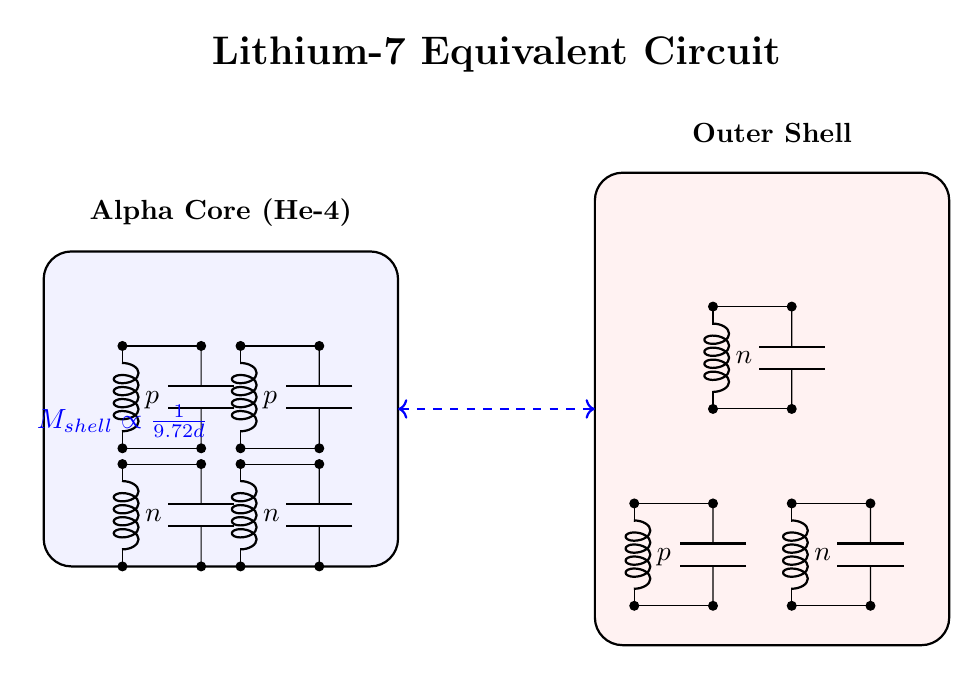
\begin{tikzpicture}
    \def\tank#1#2#3{
        \begin{scope}[shift={(#1)}]
            \draw (0,0.3) to[L=$#3$, *-*] (0,-1.0);
            \draw (1,0.3) to[C, *-*] (1,-1.0);
            \draw (0,0.3) -- (1,0.3);
            \draw (0,-1.0) -- (1,-1.0);
        \end{scope}
    }
    
    % Alpha Core
    \draw[rounded corners=10pt, fill=blue!5, thick] (-1,-1.5) rectangle (3.5,2.5);
    \node at (1.25, 3) {\textbf{Alpha Core (He-4)}};
    
    \tank{0,1}{1}{p}
    \tank{1.5,1}{2}{p}
    \tank{0,-0.5}{3}{n}
    \tank{1.5,-0.5}{4}{n}
    
    % Outer Shell
    \draw[rounded corners=10pt, fill=red!5, thick] (6,-2.5) rectangle (10.5,3.5);
    \node at (8.25, 4) {\textbf{Outer Shell}};
    
    \tank{7.5,1.5}{5}{n}
    \tank{6.5,-1}{6}{p}
    \tank{8.5,-1}{7}{n}
    
    % Loose Mutual Coupling
    \draw[<->, dashed, blue, thick, out=0, in=180] (3.5, 0.5) to (6, 0.5) node[midway, above] {$M_{shell} \propto \frac{1}{9.72d}$};
    
    \node at (4.75, 5) {\Large \textbf{Lithium-7 Equivalent Circuit}};
\end{tikzpicture}
\end{document}
